\documentclass[a4paper,11pt]{ltjsarticle}
% 数式
\usepackage{amsmath,amsfonts}
\usepackage{bm}
% 画像
\usepackage{graphicx}
\usepackage{circuitikz}
\usepackage{amsmath,amssymb}
\usepackage{siunitx}
\usepackage{float}
\usepackage{tikz}
\usepackage{askmaps}
\usepackage{multirow}
\usepackage{bigstrut}
\usepackage{slashbox}
\usepackage{rotating}
\usepackage{listings}
% 数式
\usepackage{physics}
\usepackage{mathtools}
% 画像
\usepackage{subcaption}
% 表
\usepackage{makecell}
% その他
\usepackage{url}
\usepackage{ascmac}
\usepackage{cases}
\usepackage{here}
\usepackage{upgreek}
% 日本語対応
\usepackage{luatexja}
\usepackage{luatexja-fontspec}

\AtBeginDocument{\RenewCommandCopy\qty\SI}


\definecolor{commentgreen}{RGB}{0,200,0}
\definecolor{eminence}{RGB}{120,80,250}
\definecolor{weborange}{RGB}{255,165,0}
\definecolor{frenchplum}{RGB}{10,150,200}
\definecolor{commentgreen}{RGB}{0,200,0}
\definecolor{eminence}{RGB}{120,80,250}
\definecolor{weborange}{RGB}{255,165,0}
\definecolor{frenchplum}{RGB}{10,150,200}

\lstset{
        language = {C},
        basicstyle = \ttfamily\small,
        keywordstyle=\color{eminence}\ttfamily\bfseries,
        commentstyle=\color{commentgreen}\textit,
    identifierstyle=\color{black}\ttfamily,
        xleftmargin=.35in,
        frame=lines,
    showstringspaces=false,
        numbers=left,
        stepnumber = 1,
        breaklines=true,
        numberstyle = \ttfamily\normalsize,
    tabsize=4,  
        emph={int, int8_t, int16_t, int32_t, int64_t, uint8_t, uint16_t, uint32_t, uint64_t, char, double, float, unsigned, void, bool},
        emphstyle={\color{blue}}, 
        morekeywords={>, <, ., ;, +, -, *, /, !, =, ~},
        breakindent = 10pt, 
        framexleftmargin=10mm, 
        columns=fixed,
        basewidth=0.5em,
        }

% 特定のスタイル設定
\lstdefinestyle{customtxt}{
  basicstyle=\ttfamily\footnotesize,
  backgroundcolor=\color{lightgray},
  frame=single,
  breaklines=true,
  columns=fullflexible,
  showspaces=false,
  showstringspaces=false,
  showtabs=false,
  tabsize=4,
}

\newcommand{\fig}[4]{
    \begin{figure}[htbp]
      \centering
      \includegraphics{./image/#1}
      \caption{#2}
      \label{fig:#3}
    \end{figure}
  }
\begin{document}

\title{レジスタ機械}
\author{古城隆人}
\date{\today}
\maketitle
\newpage
\section{目的}
レジスタ機械がどのように動作するかを理解する。
\section{課題内容}
課題内容を以下に示す。
\begin{figure}[htbp]
    \centering
    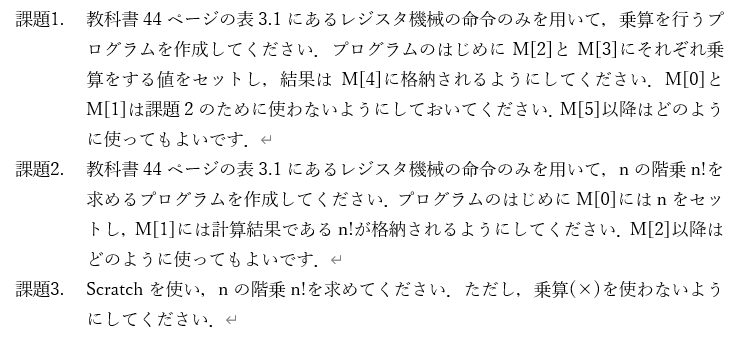
\includegraphics[width = \columnwidth]{./image/image.png}
    \caption{課題内容}
    \label{fig:kadai}
\end{figure}
\section{課題1}
課題1のプログラムをリスト\ref{kadai1src}、実行結果をリスト\ref{kadai1res}に示す。
\begin{lstlisting}[caption = 課題1のプログラム,label = kadai1src]
SETC 2
STORE 2
SETC 3
STORE 3
LOAD 2
JZERO 30 //HALT
LOAD 4
ADD 3
STORE 4
LOAD 2
PRED
STORE 2
JUMP 10 //JZERO
HALT
\end{lstlisting}
\begin{lstlisting}[caption = 課題1の実行結果,label = kadai1res]
  C:\Users\kojor_fyn5sjo\Documents\GitHub\report\2024_3IE_report\計算モデル\RM-simulator>a.exe mul.rm
 ___________________________________________
 Cycle=3530
  IC[7046]  IR[HALT 50341889]  Acc【  0】
 ___________________________________________ 
              M ----------
              |  0 |   0 |
              |  1 |   0 |
              |  2 |   0 |
              |  3 |   3 |
              |  4 |   6 |
              |  5 |   0 |
              |  6 |   0 |
              |  7 |   0 |
              |  8 |   0 |
              |  9 |   0 |
              | 10 |   0 |
              ------------

\end{lstlisting}
\section{課題2}
課題2のプログラムをリスト\ref{kadai2src}、実行結果をリスト\ref{kadai2res}に示す。
\begin{lstlisting}[caption = 課題2のプログラム,label = kadai2src]
  SETC 5
  STORE 0
  SETC 1
  STORE 1
  LOAD 0
  PRED
  JZERO  52//HALT
  STORE 0
  SUCC
  STORE 2
  LOAD 1
  STORE 3
  LOAD 2
  JZERO 42 //fin
  LOAD 4
  ADD 3
  STORE 4
  LOAD 2
  PRED
  STORE 2
  JUMP 26 //JZERO
  LOAD 4
  STORE 1
  SETC 0
  STORE 4
  JUMP 8
  HALT
\end{lstlisting}
\begin{lstlisting}[caption = 課題2の実行結果,label = kadai2res]
  C:\Users\kojor_fyn5sjo\Documents\GitHub\report\2024_3IE_report\計算モデル\RM-simulator>a.exe factorial.rm
  ___________________________________________
  Cycle=180
   IC[ 54]  IR[HALT   0]  Acc【  0】
  ___________________________________________    
               M ----------
               |  0 |   1 |
               |  1 | 120 |
               |  2 |   0 |
               |  3 |  60 |
               |  4 |   0 |
               |  5 |   0 |
               |  6 |   0 |
               |  7 |   0 |
               |  8 |   0 |
               |  9 |   0 |
               | 10 |   0 |
               ------------
 
\end{lstlisting}
\section{課題3}
課題3はスクラッチで作成したものなのでプログラムを画像\ref{fig:kadai3}に示す。
実行結果を画像\ref{fig:kadai3res}に示す。
\begin{figure}[htbp]
  \centering
  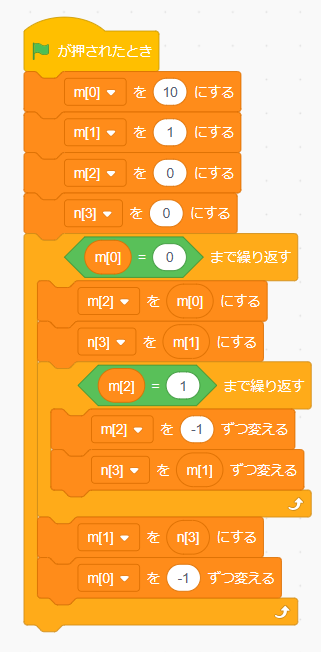
\includegraphics{./image/kadai3.png}
  \caption{課題3のプログラム}
  \label{fig:kadai3}
\end{figure}
\begin{figure}[htbp]
  \centering
  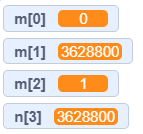
\includegraphics{./image/kadai3res.png}
  \caption{課題3の実行結果(ACC = 10)}
  \label{fig:kadai3res}
\end{figure}
\end{document}